\chapter{Strategic Analysis}

\begin{quotation}
    \textit{In war, the morale is to the physical as three is to one.} \\
--Napoleon Bonaparte
\end{quotation}

\medskip

\begin{quotation}
\textit{In Technological War, organization and leadership is to the morale as six is to three.} \\
--Possony, Pournelle, and Kane.
\end{quotation}

\medskip

\begin{quotation}
\textit{The starting point for strategy must not be that which is possible; we must discover what is necessary and try to achieve it.} \\
--General d'Armee Andre Beaufre
\end{quotation}

\begin{mdframed}[backgroundcolor=black!10]
\textbf{Note to the Second Edition:}
The first edition of this book was part text and part polemic: the strategic situation in 1969 was at a low ebb, and the threat from the Communist Empire was large and growing. Since that time there have been some beneficial changes. The United States began to take seriously the Technological War. Although the Soviet Union continued to engage in Technological War, the US stayed just far enough ahead to prevent a decisive advantage. The Reagan Administration shuttered the Communist 'window of opportunity', while internal stresses within the Communist Empire continued to grow.

The small computer, itself a fall-out benefit from military research and development (for on-board missile guidance systems), had a near decisive impact: a power without computational resources in an era of "computational plenty" suffered a great handicap. On the other hand, it was impossible for the Soviet Union to introduce the small computer and maintain the management and control of information. Arthur Koestler pointed out in 1946 that the necessary and sufficient condition for the end of totalitarian tyranny was the free flow of information and ideas within the totalitarian society. The small computer, as the ultimate instrument of samizdat, makes information control impossible.

The Soviet Union was thus presented with an impossible set of choices: introduce modern technology, and thus inform the Soviet population of the true conditions both abroad and within the Empire; or suppress that technology, and forfeit its benefits.

Brezhnev chose the latter course. Andropov and his protégé Gorbachev, possibly because as KGB officials they were acutely aware of the internal problems of the Empire, chose the former. The repercussions of that decision are nowhere near over: as we write this, there are riots in Bohemia, and a new Prague Spring -- if not a new Defenstration of Prague -- appears likely.

The other key decision was the U.S. venture into SDI: that is, a decision to open a 'second front' in the Technological War. This intensified the dilemma described above.

As a consequence of these changes in world circumstances, much of the specific analysis in this and other chapters is no longer applicable. On the other hand, the principles on which that analysis was based have not changed one whit. Winning the Technological War is as vital as ever: we must not forget that \textit{perestroika} and \textit{glasnost} are not acts of kindness, but strategic decisions which allow the Soviet Union to continue its efforts in the Technological War.

We have partially revised the text in this chapter, but much of it remains as it was written in 1968-69. We wish to repeat: circumstances change, but principles do not; and if some of our text now appears to rail against problems already solved, we hope the reader will recall that this book played its part in solving them. STP, JEP, \& FXK, Fall, 1989
\end{mdframed}

As we have repeatedly stated, the Technological War must be fought as are other wars; that is, it must be fought according to a strategy. A general who simply muddles through, overcoming each obstacle as it comes to him, fighting battles at the dictation of the enemy, and preparing only for battles already fought would soon lose the war. Yet, too often it is thought that the Technological War, which may be the most decisive engagement in the history of mankind, can be fought with precisely this technique. Technology is made the driving force, dictating to strategy; and strategy is conceived of as the employment of systems already created by the technologists, that is, strategy is confined to operational decisions. This is akin to allowing the munitions manufacturer to decide the conduct of the war.

Proper conduct of the Technological War requires that strategy drive technology; that there be an overall strategy of technology, not merely strategic elements which make use of the products of technology. Instead of the munitions designer controlling the conduct of the war, it must be in the hands of those who understand technological warfare; and this requires that they first understand the nature of war.

Lest we be misunderstood, we wish to underscore the following point most forcefully: we do not say that scientists must somehow create a strategy for technological development. Nor do we advocate turning over the conduct of the Technological War to the average flag officer or captain of industry.

This is in fact the source of one of the major weaknesses of the West in the Protracted Conflict: there are very few experts in technological warfare. It is hardly surprising, for there are few senior people in the United States who have ever studied strategy, and fewer of those have turned their attention to a strategy of technology.

The first edition of this book was used as a text in the War Colleges and two of the service Academies, so that at least some of the officer corps has been exposed to the concept of a technological strategy; but there are no universities teaching technological strategy or the essentials of it, and there are few apprenticeship programs.

A Brookings Institution study recognized a facet of this problem, pointing out that the senior service schools were teaching officers how to "manage' but not how to understand, let alone develop, strategies and fight wars. This is being partly overcome by programs such as the USAF "Warrior" and the National Defense University computerized war games, but we have a long way to go.

One of the problems of the United States is our quaint belief in the administrator, our belief that a man capable of governing a large automobile company will be a good strategist and can safely be entrusted not only with the titular leadership of the services but with a dictatorial power over them extending to the silencing of all verbal opposition. We have coupled this promotion of administrators or executives with a tendency to centralize all decision processes, particularly those involving budgets and funding. These beliefs were the major architects of our defeat in Viet Nam. The problem is not trivial.

\section{The Creation of Technological Strategy}
To illustrate what is meant by a strategy of technology, we will trace the steps in the creation of military technology; and we mean by military technology those systems which are used in the Technological War, not merely weapons. Laboratories are an obvious example of tools of the Technological War that are not weapons. Others could include logistics systems; civilian hardware useful for the nation building mission; irrigation systems and sea water conversion plants; agricultural techniques and equipment. The list is endless.

We also wish to emphasize something very strongly: we are not proposing the creation of new layers in the decision process. We do not intend this analysis of organizations for rehumanizing strategy and generating a strategy for the Technological War to be taken as recommendations for creating new organizations for solving the wrong problems, and new structures to be added to the old.

What is needed is a fundamental restructuring of the entire decision process to allow government of the Technological War according to a strategy, rather than by a series of independent technological or scientific decisions. Once strategy governs the decision process, many of the present delays are likely to vanish. They must be made to do so. Time is the most important dimension of the Technological War, both to maintain the necessary lead and to save money.\footnote{The first edition of this book proposed a number of changes in decision structure. Some of those were made in the 1980's.}

\section{The Elements of Technological Strategy: An Overview}

% \usepackage{color}
% \usepackage{rotating}
% \usepackage{tabularray}
\definecolor{Silver}{rgb}{0.752,0.752,0.752}
\begin{table}
\centering
\caption{CHART 9: Strategic Analysis}
\begin{tblr}{
  row{odd} = {Silver},
  row{3} = {c},
  cell{1}{1} = {r=4}{},
  cell{1}{2} = {c},
  cell{1}{3} = {c},
  vlines,
  hline{1,5} = {-}{},
  hline{2-4} = {2-3}{},
}
\begin{sideways}\textbf{Strategic Analysis}\end{sideways} & \textbf{Government Support}                                                                                                                                                                                                                                                                                                                     & \textbf{Technology}                                                                                                                                                                                                                                                                                                                                                                                                                                                                                                                           \\
                                                          & {\labelitemi\hspace{\dimexpr\labelsep+0.5\tabcolsep}Leadership\\\labelitemi\hspace{\dimexpr\labelsep+0.5\tabcolsep}Budget\\\labelitemi\hspace{\dimexpr\labelsep+0.5\tabcolsep}Grand Strategic\\\phantom{\labelitemi}\hspace{\dimexpr\labelsep+0.5\tabcolsep}Decision Process\\\labelitemi\hspace{\dimexpr\labelsep+0.5\tabcolsep}Public Morale} & {\labelitemi\hspace{\dimexpr\labelsep+0.5\tabcolsep}Science\\\labelitemi\hspace{\dimexpr\labelsep+0.5\tabcolsep}Research\\\labelitemi\hspace{\dimexpr\labelsep+0.5\tabcolsep}Engineering\\\labelitemi\hspace{\dimexpr\labelsep+0.5\tabcolsep}Production\\\labelitemi\hspace{\dimexpr\labelsep+0.5\tabcolsep}Management\\\labelitemi\hspace{\dimexpr\labelsep+0.5\tabcolsep}Procurement\\\labelitemi\hspace{\dimexpr\labelsep+0.5\tabcolsep}System Analysis}                                                                                   \\
                                                          & \textbf{Non Military Conflict}                                                                                                                                                                                                                                                                                                                  & \textbf{Military Arts}                                                                                                                                                                                                                                                                                                                                                                                                                                                                                                                        \\
                                                          & {\labelitemi\hspace{\dimexpr\labelsep+0.5\tabcolsep}Psychological Operations\\\labelitemi\hspace{\dimexpr\labelsep+0.5\tabcolsep}Economics\\\labelitemi\hspace{\dimexpr\labelsep+0.5\tabcolsep}Trade\\\labelitemi\hspace{\dimexpr\labelsep+0.5\tabcolsep}Diplomacy\\\labelitemi\hspace{\dimexpr\labelsep+0.5\tabcolsep}Internal Security}       & {\labelitemi\hspace{\dimexpr\labelsep+0.5\tabcolsep}Strategy\\\labelitemi\hspace{\dimexpr\labelsep+0.5\tabcolsep}Intelligence\\\labelitemi\hspace{\dimexpr\labelsep+0.5\tabcolsep}Counterintelligence\\\labelitemi\hspace{\dimexpr\labelsep+0.5\tabcolsep}Logistics\\\labelitemi\hspace{\dimexpr\labelsep+0.5\tabcolsep}Operations\\\labelitemi\hspace{\dimexpr\labelsep+0.5\tabcolsep}Command\\\labelitemi\hspace{\dimexpr\labelsep+0.5\tabcolsep}Military Analysis\\\labelitemi\hspace{\dimexpr\labelsep+0.5\tabcolsep}Non Violent Warfare} 
\end{tblr}
\end{table}

The elements of technological strategy are shown on Chart 9. It will be seen that the heart of the process is something we call strategic analysis. In other times this was called War Plans; for the Technological War the scope of analytical work must be broader than that of the old War Plans division of the European General Staffs. Strategic analysis is a process which generates a plan: it seeks the proper use of available and future weapons of the Technological War, orchestrates them, and produces the actual engagements. These may take the form of research plans, hardware construction, intelligence operations, or even military battles. The latter are unlikely in a Technological War until one side has achieved a decisive advantage.

At the top of the structure is the political leadership of the nation. This element makes resources available, particularly funding. It sets the grand strategy of the nation -- that is, whether the nation is to go on the offensive or defensive, be expansionist or static, be interventionist or isolationist, and so forth. In addition, the political leaders must support the personnel engaged in the Technological War. It must be concerned not only with the morale of the technological soldiers but with the nation at large, justifying the necessary expenditures, explaining the purposes of each approach taken, and combating indifference and defeatism. Unless the political leaders properly perform their mission, the Technological War cannot be won.

The second major element in the creation of a strategy of technology is what is called the military arts. This includes subelements such as commander, strategists, and intelligence personnel. They must understand the significance of the moves made by the enemy in the Technological War, and formulate strategies for overcoming them. For example, if the enemy decides to engage in warfare, open or covert, at a level of hostility where the United States is weak, the military strategists must have available contingency plans for changing the nature of the war, either through controlled escalation or otherwise, to a kind of war in which we dominate. The military strategist must have an appreciation of our capabilities and limits as well as those of the enemy, and he must continually revise his estimates of what modern technology can accomplish.\footnote{This process has in part been implemented since the first edition of this book. The result is known as competitive strategies.}

nologists, both scientists and engineers, obviously are essential to the Technological War at this point. Through independent research, they create new technology which may or may not be useful in the conduct of the technological conflict. They discover scientific laws and principles which may be exploitable as military or nonmilitary weapons. They should be guided in their research by the requirements of the military, by the military roles and missions that require improvements or that have been conceived of but cannot as yet be performed.

Others will be engaged in pure research which may or may not be useful in the Technological War but is beyond the charter of the strategist to direct or control. However, while we recognize the value of pure research, such as that carried out by Einstein and Fermi, we note that the creation of military technology from their physical principles was the result of a directed effort. We do not advocate over-control and micro-management of the research process and scientists in projects funded by DOD; however, some direction and control is necessary.

Modern technology is fluid; often specific items of technology can be created on demand through focusing of effort. The Soviet Union employs this method consistently to preserve resources, and has achieved many notable successes despite a paucity of reserouces compared to the West. In the United States the development of the hydrogen bomb, a key event in preserving the freedom of Western Civilization, was largely the creation of a focussed effort despite the fact that it was unwanted by many scientists, some of whom believed it unfeasible.

We want to be understood clearly: scientific research and discovery are in large measure products of free inquiry and human freedom. This fundamental point has been confirmed in a dramatic manner by the performance of the U.S.S.R., which depends to a surprisingly large extent upon the pure science produced in the Free World, but which, within the limits of its capabilities, has had an astonishingly good performance in the military applications of scientific discovery.

No one can predict the ultimate use of any research in any of the pure sciences. Except for navigation, astronomy was of no military use before the space age. Yet the mathematical techniques developed by the astronomers to solve the four-body problem helped to overcome one of the greatest difficulties in antiaircraft defense. Therefore, as a general principle, no scientific investigations should be starved, let alone suppressed. However, those researches that appear to have no strategic utility and most probably will not be useful for several decades surely need not be accelerated or be given priorities -- even though they may be of extreme utility in the next century. It would be entirely sufficient to allow such work to proceed at a normal pace.\footnote{Times change, of course; what was 'far out' in 1969 became vital in 1980. In the chapter "Assured Survival" this book in 1969 advocated strongly focused efforts into 'beam technologies'. That research paid off handsomely after 1983; but note that beam technology is only one of the means for constructing viable missile defense systems.}

s that many lines of basic research can be safely regarded as of great strategic importance, even though we may be unable to predict specific applications. For example, the steady exploration of atomic particles may, in the end, yield no strategic value, but the overwhelming odds are that a better understanding of the structure of matter will result in entirely new tools and materials. Discoveries in medicine, biology, psychology, and agriculture could have massive impacts on strategy.

Hence we believe this to be a matter of common sense: first, to support particularly those lines of pure research which promise an early strategic payoff; second, to regard technology as a task and end-product of all sciences; and third, to devote far more time and resources to analyzing research discoveries from the point of view of their possible strategic utility. In other words: do not hamper any research; support heavily research that has a predictable payoff; and reduce uncertainty concerning the military and strategic usability of scientific discoveries.

Note that the ordering of priorities is itself a strategic decision. When the threat is small and waning, one wished to allocate resources to technologies which may not mature for many years; when the threat is large and growing, technologies of more immediate application are needed. These are not scientific decisions.

The technological community has several duties. These will be discussed in more detail in later sections. For the moment, they can be summarized as shown on Chart 10.

The final major source of technological strategy is the nonmilitary conflict expert. The traditional elements of this community, namely, the diplomatic corps, foreign aid experts, propaganda and psychological warfare experts, and economic warfare practitioners, have a self-explanatory role. The important point is that this group cannot be ignored; and perhaps even more important, they cannot operate in isolation. Trade agreements, diplomatic negotiations, and political alliances are extremely important facets of Technological War, and the efforts of those engaged in these aspects of the Protracted Conflict must be coordinated according to a strategy. It cannot be stated too strongly that the Treaty of Moscow and the whole test-ban affair was a great Technological War victory for the U.S.S.R. To a lesser extent, U.S. trade policies have also been Soviet victories in the Technological War, in that they have allowed the Soviets to concentrate their scarce technological talent on military systems in the confident expectation that the West will sell to them the technology and technological products the rest of their economy requires.\footnote{This situation is essentially unchanged in 1989; the USSR expects \textit{glasnost} and \textit{perestroika} to produce internal changes, but also to induce the West to loosen up restrictions on both strategic goods and credit. While it is important to "give Gorbachev a chance" it is also vital that we don't preserve and increase Soviet military power. In the 1990's Trade policy has become the key front for the Protracted Conflict. [1987]

The decisive moment was when Reagan refused to abandon SDI at Gorbachev’s request. This threatened to make obsolete the extremely expensive missile establishment of the USSR; the cost of refurbishing that system to make it viable in an era of strategic defense was unthinkably high for USSR planners. The alternative of using it before it became obsolete was no more attractive due to NATO readiness (although there certainly were advocates of a ‘take Europe now’ policy within the PolitBuro.)}

This section has been an overview of the creation of technological strategy. In the following sections, we turn to each contributor in detail and trace the development of new weapons systems.

\begin{mdframed}[frametitle={CHART 10: Duties of the Technological Community}]
    \begin{itemize}
        \item Providing Strategic Analysis with new possibilities.
        \item Developing specific systems from military requirements.
        \item Creating technology on demand.
        \item Creating technology from pure research.
        \item Discovering new fields of technology.
    \end{itemize}
\end{mdframed}

\section{The Creation of Military Technology}

In this analysis we have divided the creation of technology into three phases but we caution the reader that their linear form is in part illusory. Many of these functions are carried out simultaneously, and it is not necessarily true that all systems will pass through all stages we have shown. However, it will be helpful to trace all steps in the process, keeping in mind that this is not intended to be a recommendation for new delays in decision making. We do not insist that each technological creation go through these steps in succession.

In the discussion that follows we are attempting to show the kind of analysis which should be followed in order to coordinate technology with strategic planning. This is in no way a description of the actual steps taken in present weapon system design; indeed, as demonstrated in earlier chapters, we argue that at present there is no automatic review of technology to determine its relationship to the overall plan of action in the Technological War. Instead, decisions are made at present on the basis of technological or scientific factors, and usually by scientists.

\begin{mdframed}[backgroundcolor=black!10]
Circumstances change: in 1989 this is no longer true. Now decisions are made largely on the basis of cost, with a heavy dose of political pork barreling from the Congress. There is, however, some appreciation of the need for a technological strategy, and to that extent the situation is much better now than in 1969.
\end{mdframed}

\section{Phase 1}
The first phase of the creation of military technology is shown on Chart 11. It begins with a strategic appreciation. This was once part of the intelligence process. In the 1960's and 70's the intelligence community was largely confined to the provision of data and descriptions of foreign technology to policy makers. The policy makers were generally civilians with little experience in the conduct of war, and rely on staff assistants for advice. The reorganization of the services divorced the top military staffs from direct participation in the operation of the services themselves, which are organized into commands and function as nearly self-contained structures under the direct orders of the Secretary of Defense. During the McNamara era the Plans and Doctrines departments of the various military service headquarters were thus required to compete for the attention of the civilian policy makers who alone have the authority to implement changes in the organization and structure of military forces.

\begin{figure}[h!]
    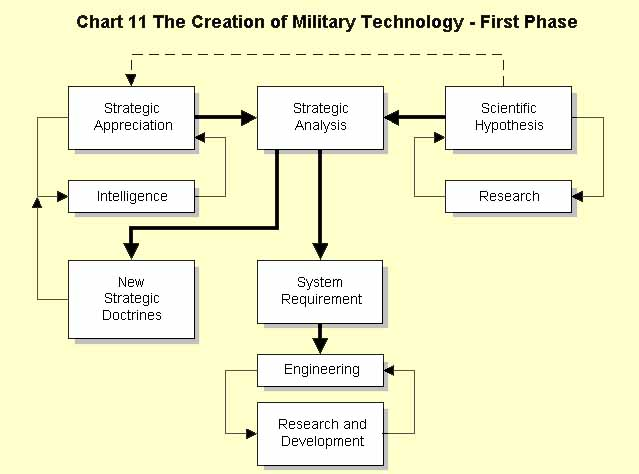
\includegraphics[width=\textwidth,height=\textheight,keepaspectratio]{./chart-11.jpg}
    \label{fig:chart-11}
\end{figure}

For much of the 60's and 70's there was thus no organization in the United States whose mission was to prepare a strategic appreciation. This serious defect in our national policy machinery, but was not likely to be observed by the average civilian official because strategic appreciation had nearly become a lost art; and one does not feel the need for something he has never seen or known about.

Prior to the McNamara Era, the JCS had the responsibility for strategic assessment, but that role was eliminated by the civilian 'Whiz kids' he brought into the Pentagon. The role is being restored under the Goldwater Act.

All military technology should begin with strategic appreciation. Unlike an intelligence report, an appreciation takes into account our own resources and weaknesses, enemy objectives and intentions, our own goals and policies, and alternatives available to us. It provides an estimate of the situation, and a prediction of the outcome of the engagement if existing trends continue.

As are all military assessments and decisions, strategic appreciation is an art. It is more than what an economist or physicist would call an analysis or evaluation. Strategic appreciation requires a feel for events and trends which can be gained only from historical knowledge and experience of the proper kind; and that experience must include living in an environment in which one is constantly aware of the opposition of an intelligent enemy. Business and scientific expertise are not enough; almost every skilled generator of strategic appreciation is a military officer of long service, although not every senior officer is capable of an appreciation of the situation in the Technological War. One excellent example of an officer who possessed the talents required for this work was General Bernard Schriever, whose work in generating Project Forecast and Project 75 has been noted throughout this book.\footnote{The era of computational plenty has had many beneficial effects, but it has one major drawback: if not careful, one can easily exaggerate the accuracy of computer predictions. The output of a computer analysis is really no better than the understanding of the programmer who built the analytical model; and since even today's computers can't understand history and economics and leadership personalities, they output of a computer simulation isn't likely to be an accurate prediction of world events. As an example, a popular computer game called "Balance of Power" is often used in university classes on foreign relations, and has been used in the Foreign Service schools. This game ignores economics and trade, and is largely "won" if the U.S. player pursues a policy of appeasement vis-à-vis the 'implacable' Soviet Union. Nothing the U.S. player can do will make fundamental changes within the structure of the Soviet player's empire. Balance of Power is an amusing game, but it is a pernicious instructor in real-politik. [1989]

We note that had the US followed the precepts of that game—which was based on the principles then taught by the Department of State—the Seventy Years War or Cold War would still continue. [1997]}

The strategic appreciation provides the strategist with an estimate of the probable outcome of present trends, and allows him to form judgments about the future requirements and capabilities for military technology. It thus forms the first element of strategic analysis, but by itself it is insufficient. The second element comes from the scientific and engineering communities in the form of possible or probable developments in the world of technology.

It is important to note that scientists and engineers will in general produce fundamentally different kinds of inputs. Scientists' reports will generally be given as scientific hypotheses, and insight and experience on the part of the strategist are required to see the implications in terms of new weapons systems capabilities.

Engineering reports are generally more concerned with short term problems, costs, and schedules. The technologies they advocate will have less scientific uncertainty -- you can be fairly sure they can build what they say they can -- but will also tend to be less imaginative if more immediately practical. Determining wheter to invest resources in science or in engineering development is one of the key decisions of the technological war. For example: the scientific work of Arthur Kantrowitz at the Avco/Everett Research Center, was crucial to the development of the continuous wave laser. Kantrowitz was dismissed as a dreamer by many in the aerospace community, who claimed in 1960 that lasers would never be practical military weapons because they could never be made more than 5% efficient.

Technology will have two distinct impacts on military systems: it will identify new uses for our own systems and suggest new capabilities that would be desirable for the force; it will also postulate potentially new enemy capabilities against our force, generating new requirements for ourselves and changing the predicted outcome of future battles.

\section{MIRV: An Historical Example}

Note to Second Edition:
After extensive debate, the United States under Nixon decided to deploy MIRV, Multiple Independently Retargetable Re-entry Vehicles. This was a key event in the Technological War. In 1969 when the following was written, that decision had not been made, and there were strong advocates against MIRV deployment: that it should either be left as a pure R\&D effort, or abandoned altogether.

Fortunately the U.S. continued MIRV development and actual deployment. If we had not done so the consequences would have been extremely serious.

\begin{mdframed}[backgroundcolor=black!10]
\textbf{Note to the Second Edition:}
After extensive debate, the United States under Nixon decided to deploy MIRV, Multiple Independently Retargetable Re-entry Vehicles. This was a key event in the Technological War. In 1969 when the following was written, that decision had not been made, and there were strong advocates against MIRV deployment: that it should either be left as a pure R\&D effort, or abandoned altogether.

Fortunately the U.S. continued MIRV development and actual deployment. If we had not done so the consequences would have been extremely serious.
\end{mdframed}

As an example, the implications of MIRV have an impact on both offensive and defensive systems. If MIRV is installed only in offensive weapons, this technological development can allow the utter destruction of a second strike force before it is launched, without the attacker having to deploy any new missiles. An aggressor could thus construct a full first-strike capability in his territory without doing anything observable by satellites or radar. As no intelligence organization in the world can guarantee that a potential aggressor is not altering the warheads of its existing force to take advantage of MIRV technology, MIRV poses a distinct new threat to U.S. missiles, and thus to the survival of the nation.

MIRV also has the effect of multiplying the capability of the surviving boosters in a second-strike force, by allowing each surviving missile to destroy more than one enemy target. It could, therefore, aid the defense as well as the offense. The actual changes in the strategic equation are dependent on additional factors, in particular the improvements of the yield-to-weight ratio of nuclear weapons (lighter weapons with a bigger bang allow installation of more MIRVs in a given booster), and improvements in accuracy (the more accurate the MIRV, the better chance that the second-strike force will be destroyed completely). In contrast to MIRV, extremely high accuracy of intercontinental missiles chiefly aids the offense: that is, great accuracy is not needed to destroy a city, but accuracy improvements allow the first strike to eliminate a greater proportion of the defender before he can launch a counter blow.

\begin{mdframed}[backgroundcolor=black!10]
A current example would be the debate over strategic defenses. SDI forces both sides to stretch their technological resources to the limit. This is clearly advantageous to the U.S. because we have more technological resources: SDI deployment at the very least forces the USSR to spend its resources refurbishing its Strategic Offensive Forces rather than adding new capability to the SOF. They probably cannot afford to do this, which forces the Soviet leadership to decide whether a large and expensive SOF is needed at all. (1987)
It is now clear that the above analysis was correct. (1997)
\end{mdframed}

The strategic analyst must understand the implications of new technology, and the uses to which they may be put in both the Technological War and the Protracted Conflict. His analysis must extend beyond such obvious areas as improvements in missile guidance and accuracy to more subtle developments based on new scientific principles. He must also be ready to exploit fallout benefits, such as small computers.

The strategic analyst also uses the strategic appreciation to guide research efforts. From military requirements for underseas warfare capabilities, the technological community may be encouraged to do research in oceanology, particle propagation in dense media, measurement of cosmic ray backscattering, or examination of surface phenomena. Research budgets will to a great extent be controlled by the priorities for new technology set by the strategic appreciation.

However, it bears repeating: only a fool would so trust his own judgments as to cut off lines of research sponsored by competent scientists who believe themselves on the threshold of new principles or new fields of scientific endeavor. Research programs must always hedge against improper judgment or faulty analysis, but they must not be allowed simply to proliferate according to the specialties of the scientists who happen to be employed.

In fine, a technological "center of gravity" must be chosen, and research priorities allocated around it, so that most of the programs contribute to, or are designed to make use of, the advances in the chosen field of emphasis. Research in unrelated fields is good insurance, and should be carried out; but no one spends the major part of his budget on insurance to the detriment of his own plans.

The strategic appreciation and the technological state of the art are then analyzed in the light of the requirements of the other members of the Technological War community. Restraints imposed by political authority and diplomatic necessity must be considered, while, equally importantly, the effects of those restraints on the Technological War must be made clear to policy makers. There are times when diplomatic policies can be overcome only through enormous technological effort, such as in the case of the Test Ban; in these instances, policy makers should at least be made aware of the problems involved in the policy so that they will know their true costs to national security as well as their benefits.

When the restraints have been set and the requirements for the force understood, a technological strategy can be generated. It must plan for maximum strategic surprise, and incorporate planning for technological pursuit. It must plan for real options as well as paper options -- that is, for systems that can be built and deployed as well as those that are only theoretical possibilities dependent upon the success of high-risk research and development. The strategic plan must provide for flexible systems which can incorporate new technological developments expected in the near future, and for defense against possible enemy capability improvements.

This analysis will generate a set of military system requirements. These will be brief descriptions such as "a general-purpose offense-defense missile system capable of using many elements in common for both missions. The offense system should have intercontinental range, and the defense system should be capable of interceptions in either the upper atmosphere or mid-course flight at ranges of at least 800 miles from the interceptor launch site." It is, in other words, a strategic system concept. In a real world case, the performance requirements would be defined more rigorously but not in detail. The strategic analyst is concerned with establishing a requirement, not with the actual design of technology.

\begin{mdframed}[backgroundcolor=black!10]
We understand that the requirements process is more complex than this. The requirements game is also used as a primary way to suppress promising lines of research and development.
\end{mdframed}


The system design description is turned over to the engineers and technologists for implementation. Some performance features can be implemented with off-the-shelf hardware. Others require new developments in technology. Research will be required to provide a system design. This, however, is directed research to solve specific problems and provide specific technology building blocks to achieve the desired system performance. The engineering design team will also generate a series of estimates of system performance traded off against time and money; that is, an estimate of how long and what cost will be required to achieve each of several different levels of performance. Often this will be accompanied by proposals for alternative approaches to solve the technical problems. These estimates are returned to the technological strategist for decisions.

The decision as to which of several competing technical approaches should be used, or whether to spend the time and effort to achieve a particular level of performance instead of using cheaper methods to build systems of less value, will be one of the most important decisions in the life of the weapon system. Such decisions should be made with due regard to strategic necessities, not merely their scientific elegance. For example, a strategist may require an operational system within a certain period to assure national survival; the possibility that a greatly superior system will be available at a later date may be interesting, but it is irrelevant. He may also be able to restructure his existing forces to provide a stop-gap defense which will carry him over to the period in which the more advanced system will be available, or even decide to abandon the system altogether in favor of a different method of achieving security. The point is, those are strategic decisions, in which technologists and scientists participate only as generators of information, not as part of the policy-making process.

Decisions at this stage must often be referred to political authorities at the highest level. When this is done, the strategic analyst must be able to provide them not only with an understanding of the cost-performance tradeoffs but also an appreciation of the strategic necessity of various performance levels and an estimate of the magnitude of future demands for resources.

In any event, such crucial decisions should be made at a level where there is likely to be an understanding of problems of national security, not, as was the case in the McNamara era, by low-level civilian scientists who have never been faced with real military decisions. The economist in the Pentagon who wants everything reduced to a set of numerical values so that he can pick the minimax strategy has already confessed his ignorance of strategic realities, which cannot be given in numerical form.

In 1989 the decision maker is likely to be a Member of Congress, or, even more likely, a Congressional Staffer, whose expertise is more likely to be in political than strategic analysis. Micro-management and pork barreling by Congress has replaced the systems analysis by Whiz Kids in the Pentagon.

\section{Phase 2}
The decision as to system performance expectations and the technical approach to be employed begins the second phase of system development (see Chart 12). The systems engineers will work with the scientific community, seeking technological developments that may be useful to the system design and requesting assistance in research programs. Eventually, a systems proposal is generated.

\begin{figure}
    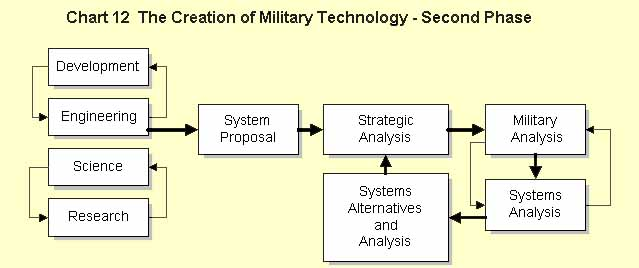
\includegraphics[width=\textwidth,height=\textheight,keepaspectratio]{./chart-12.jpg}
    \label{fig:chart-12}
\end{figure}

At this time, the specific system appears in a recognizable form. It is no longer simply a requirement for a particular mission but a hardware concept, employing radars and interceptor vehicles, warheads and guidance systems, ICBM stages and nosecones, bases and operating personnel. It is for the first time something that can be discussed by the general public, the Congress, and the average civilian official.

Note that, while this stage is usually the beginning in our present method of creating military technology, it is in fact quite late in the process. Systems proposals are expensive in terms of money and technological resources, and should not be generated merely to satisfy curiosity or because they can now be designed. They should conform to a recognizable need identified by strategic analysis.

The concept must then be examined by the military professionals who will use the system. However, if the first phase has been carried out properly, the new system will come as no surprise to the military process. We show military analysis as a separate step because it is at this stage that the system should receive a thoroughgoing review by field commanders to be sure it conforms with such realities as missions, existing installations, manpower availability, operation with other weapons, maintainability, etc. In addition, the impact of the system on force doctrines must be ascertained, and either the system adjusted to the doctrine, or the doctrines changed in time for adjustment to the system. Proper military analysis at this stage prevents the strategist from surprising his own troops -- which has happened more than once in the past -- and thus allows time to develop new employment doctrines in keeping with new capabilities.

This review may once again force a modification of the system design, and require that the system be submitted again to engineering and development, then back to the military analyst. Because of the delays inherent in this kind of process, it is obvious that the strategic analyst should be familiar with the operation of the forces, not merely be an armchair theorist, so that the first phase will identify and correct the major operational limits imposed on a new system design.

The second phase will thus evolve a system proposal that stands up. The first phase has ensured that it will be strategically useful. Military analysis ensures that it is militarily sound and will conform to the best technological data we have available. It is at this point, and not really earlier, that the systems analyst is useful. He performs tradeoff studies on performance, mission, and cost, to generate a series of alternative systems design possibilities and to compare this systems proposal with other possible ways of completing the mission. He hopes to show the effect of adopting one or another of a family of systems. Eventually a series of proposed alternative systems, not all of which have any assurance of being deployable, and an analysis of cost-performance tradeoffs are returned to the strategic analyst.

\section{Phase 3}
The strategic analyst must now exercise his own analytical judgment in consultation with the engineering and military operations experts (see Chart 13). He cannot base it simply on numerical analysis and statistics, but must take account of strategic principles and real uncertainties. Using his strategic knowledge he will reach a decision. He will select the system that offers the best strategic possibilities, including the capability to achieve surprise and pursuit, etc. There has been a policy breakthrough.

\begin{figure}
    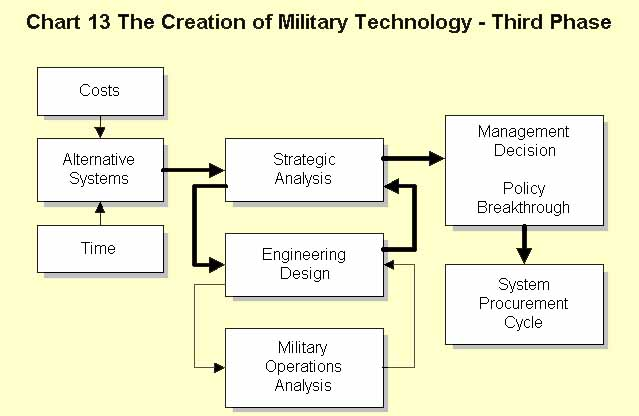
\includegraphics[width=\textwidth,height=\textheight,keepaspectratio]{./chart-13.jpg}
    \label{fig:chart-13}
\end{figure}

If the proper analyses have been carried out, and in particular if the first phase has been given the attention it deserves, the decision should not take long to make and will not be difficult to defend before strategically alert critics. Many project decisions can be made by relating them to the overall strategy of conduct of the Technological War. Others may require revision in the national strategy. The main point is that once a definite policy and strategy is accepted at the highest levels, project decisions concerning weapons systems will not be impossible for lower level commanders and can safely be entrusted to them. It is only when the top generals do not themselves know what they or their civilian superiors want done that the colonels and majors must submit even the smallest decisions to the top staff.

The system design then goes into the procurement cycle. This function is the best understood of all phases of technological development, and it is the least difficult (although the most expensive) step in the creation of military technology. In the past, procurement managers have been hampered in their work by an excess of management from the top, but to some extent this has been solved by placing a public relations expert in ostensible charge of the program, leaving the real manager (now second in command in the table of organization) to get on with the job while the "Director" uses up his time and that of his superiors in endless briefings. This strategem is more successful than might naively be assumed.

Because the procurement cycle is the best understood and most discussed of the phases of military technology, we will not discuss it here. For a brief discussion of the problems and work of the program manager, the reader is referred to a well known article by then Colonel Lawrence Skantze of the United States Air Force. The opening paragraphs are particularly worthwhile.\footnote{Colonel Lawrence A. Skantze, U.S.A.F., "The Art of the Program Manager," Air Force-Space Digest, LII, 11 (November 1969), p. 78.}

\begin{mdframed}[backgroundcolor=black!10]
Alas, since the above was written, there has been considerable change in the procurement process; due to micro management by Congress and a proliferation of regulations, procurement has become much more expensive, and takes a very great deal longer, than in 1969.
Reform of the procurement process is somewhat beyond the scope of this book; but we do note that it is a major problem for the Technological War.
\end{mdframed}

During the past ten years, the evolution of research and development (R\&D) in the Department of Defense might be characterized by two significant achievements:

The development, test, and acquisition of a substantial number of highly sophisticated, expensive weapon systems.

The development of an equally substantial number of R\&D management systems, techniques, and tools.

Since the latter is a direct outcome of the former, one might assume that the errors these tools and techniques were designed to overcome have been eliminated. In the real world of R\&D management, however, this is not always the case. Such tools as System Engineering, Configuration Management, Scheduling, Cost Programming and Control, etc., are most worthwhile. But the craftsman's skill determines the true effectiveness of the tool. Tools have been oversold to the extent that professional R\&D management-course curricula and most trade-journal articles create the impression that R\&D management is a science. The implication is that applying all of these tools as doctrinaire formula assures successful program management. This is simply not so. Program management remains more an art than a science, and anyone who believes differently should take a second look.

\section{Leadership in Technological Warfare}
The general decision path for leadership in Technological Warfare is shown on Chart 14. At present the U.S. defense decision process is not organized as shown on this chart, which represents our judgment of what would constitute a proper organizational structure for the creation of technological strategy and weapons systems.

\begin{figure}[h!]
    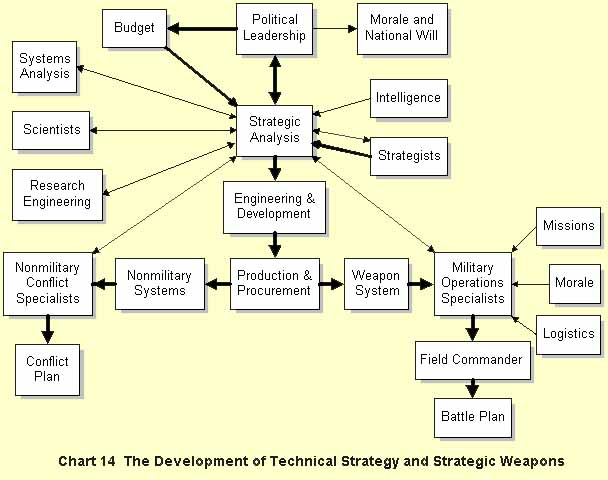
\includegraphics[width=\textwidth,height=\textheight,keepaspectratio]{./chart-14.jpg}
    \label{fig:chart-14}
\end{figure}

\section{Political Decision Makers}
The task of the political decision maker -- the civilian control of the military we hear so much about -- is to set policy and see that the grand strategy of the United States is carried out, not to function as general officers in mufti and interfere with the proper operation of the services. Civilian control of the military is important; and it is basically guaranteed in the section of the Constitution which makes the President the Commander-in-Chief of the armed services, as well as in those specifying the functions of the Congress and forbidding appropriations for the Army for more than two years. It is not civilian control to place untrained political appointees at every level of the services and require military professionals to submit all decisions to them before implementation. Such a system of political commissars was tried by the USSR with such disastrous results that we are unable to understand why the United States should institute something along those lines in our military development and procurement commands; yet that is precisely what has been done.

Secretary McNamara's "whiz kids" believed themselves competent to make almost every military decision, and to do so while also holding the privilege of disassociating themselves from the resulting disasters they had produced. Civilian management of the Vietnam War should be sufficient example for anyone, but if more examples are needed the TFX and C5A debacles are also illuminating. In 1968-69 we witnessed a shortage of military fliers caused by the civilian decision to close the schools for pilots, the lack of iron bombs in Vietnam despite the recommendations of the services, and the provision of our combat troops with more than enough turkey on Thanksgiving but not enough helicopter gun ships. Civilian control of the military is a Constitutional requirement; civilian command of the military arts is not.

The chief role of the political leader is to frame basic national goals and policies. These include such factors as whether the nation will be a stabilizer or a disturber; aggressive or defensive; isolationist or interventionist. It is also to be hoped (although from previous performance not expected) that the basic national goals will at least be consistent with each other. The President as head of the National Security Council, with consultation with the Congress as representative of the people, is the only proper level at which such broad and basic decisions can be made; and it is vital that these fundamental goals be set, for without them the strategist is helpless.

Political decisions of this kind cannot, of course, be made independently of the strategist and the technologist. Until the political authorities know what alternatives are open they cannot decide between them; the principle is that a strategy or policy should not be adopted unless it is based on real capabilities. There is no point in considering a strategy of rollback if the means for implementing it are not available and cannot be made available; and there is no point in adopting a strategy of containment if Communism cannot in fact be contained. You cannot opt for Fortress America if defense cannot be built, and you cannot be a world policeman without an effective police force. The statesman must be made aware of the options actually and potentially available and the costs and consequences of each.

There must also be hedges against a changed strategic environment. Even if national authority is convinced that the rulers of the USSR have mellowed, simple prudence requires that there be some insurance against renewed radicalism in Soviet leadership. After all, not even the highest authorities in the USSR can be absolutely sure who will be in control in years to come, or even what the structure of government will be. There must be preplanned alternatives in the event of technological surprise, whether the surprise comes from our own laboratories or in the form of enemy weapons. The one generalization that can be made with certainty about our scientific era is that it will remain uncertain; that the rapid stream of technology will bring new weapons we did not predict. A prudent national strategy will realize this elementary fact and retain sufficient flexibility to allow adjustments.

Another important but recently neglected duty of the political authorities is leadership in solidifying national morale. The political leader must understand the doctrine of Just War and be able to transmit it to the nation. Where sacrifices are called for, the statesman must make the population understand their purpose and necessity. Precisely because we are faced with a dictatorial enemy who does not need to consult his subjects before making strategic decisions, the leaders of the West must continually make clear to the people exactly what is at stake. If freedom is to survive the Technological War, this task is at least as important as the civilian control of our own military.

\section{Budget}
The budgetary process is inseparable from the political machinery of government; the concept of scientific management of the disbursement of billions of dollars extracted from the taxpayers is a myth. Indeed, the control of governmental finances is one of the most important of political decisions, and some theorists have gone so far as to say that it is the essence of politics.

In financial decisions as well as in others, the political authorities must be guided by sound strategic advice, and the strategist should have access to fiscal officials in order to determine priorities. However, strategy does not consist merely of giving the strategist all he asks for, and certainly we do not argue that the defense of the United States requires that the services be given a blank check. Civilian expenditures are obviously relevant. Then, too, military budgets are no longer sensible, and indeed are deliberately inflated. This is not because duplicity is inherent in the military services but because it has become traditional to inflate budget requests so that political officers can take credit for cutting them to trim off the fat.

The problem with this negotiatory method of arriving at budgets is that the political authorities are aware that the budget is inflated. They then seek to make cuts below the sum the military would have requested had they been presenting an honest budget. In many cases they are perfectly justified in doing so, but how can anyone be sure? Service chiefs are generally not aware of their real requirements because their own subordinates have often inflated their requests, anticipating a general trim at the chief of staff and service secretary level. The upshot is that no one is really sure which programs are vital to national security and which are not.

This kind of problem will continue in our republic, and we are hardly foolish enough to believe that we have a solution to it. So long as democratic politics exist, various stratagems must be employed by its servants. We do point out, however, that it is much easier to solve budgetary problems as part of an overall strategy than to control hundreds and thousands of individual programs; and furthermore, that there will be less need for centralized control of the myriad programs that make up defense research, development, and procurement if there is a strategy. Games and debates will continue as always, but if top-level decision makers first decide on strategic centers of gravity they will find that many of the details that plague them today will take care of themselves.

\section{Intelligence}
The intelligence function is one of the most important in the Technological War. Since this is a work on technological strategy, not on intelligence, we do not provide a lengthy discussion of the details of this vital function.

The intelligence community provides inputs to the strategic analyst as well as to political decision makers. It is of vital importance that this intelligence be reliable; indeed, it is often better to be less complete, but more reliable, than to indulge in theories. In particular, the intelligence community cannot be certain about enemy intentions, which are subject to rapid changes. The strategist must work mostly with capabilities and technological trends, and he must have a flexible general understanding of who the opponent is and will be, what the range of his intentions might be, and what he probably will not do. And he must have detailed knowledge of the opponent's operational doctrine.

Intelligence cannot ensure against technological surprise, although the United States has certainly been surprised by enemy actions that were easily predictable. Technological surprise in particular can bring about near-disasters, not the least of which is brought about by psychological effects on the population: people either despair or demand overreaction in a particular field that causes improper utilization of resources.

\section{Strategists}
As General Beaufre has pointed out, the strategist must not limit himself to what is possible; he must find ways to do what is necessary. Wishing for a technological capability will not necessarily give us one, but the history of technological development, particularly of weapons, leads us to believe that identification of a technological requirement increases the likelihood of fulfilling it.

In any research program, there will be alternatives. There is usually more than one way to reach a technological goal, and several competing principles may be involved.

Choices have to be made, and it seems to us far more reasonable to make them on the basis of strategic necessity than simple technological elegance. Cooperation between strategists, technologists, and politicians will solve almost any problem, given the resources of the United States; hostility between these groups precludes the solution even of simple problems.

Strategists are almost never found in universities, or indeed in civilian life. These rare birds will generally have had a long career of working with military officers and military problems. Most strategists are, of course, military officers of reasonably high rank and long service. The converse is not true; many high ranking officers of long service have no conception of strategy -- this is not intended as a criticism. The vast majority of military assignments involve the implementation of a strategic plan rather than its generation. Leadership of men, technical proficiency, courage, stamina, and careful attention to detail are all required of the successful field officer; yet nearly all these qualities may be lacking in a good strategist.

The strategist is, above all, an intellectual, but he is an intellectual of a different order from the scientist and engineer, or the average university professor. The strategist, unlike the scientist, deals with a world of secrecy, incomplete information, and real uncertainties which cannot be measured by statistical procedures. He lives in a world of intelligent opponents who seek to thwart him at every turn. He is concerned with the generation of plans which will be carried out by others, and he makes use of principles rather than scientific laws.

Strategists may in fact be unable to carry out their own plans. Many great strategists have lacked the vital qualities of leadership required of great military captains. Some have suffered from severe personality defects which prevented them from convincing anyone of the soundness of their plans. Consequently, strategists are not necessarily carried to the top of the military services unless they have been diligently sought and carefully chaperoned during their careers.

The U.S. armed services are not organized to locate and promote strategists, and originality in strategy has never been plentiful during out history. American military history shows rather the reverse: in all our wars, we have generally started with poor strategists in command and had to muddle through until we found strategic competence -- e.g., Lincoln's difficulties in locating a general who could take advantage of the peculiar strengths and weaknesses of the Union Army.

Consequently, we will not generate a strategy of technology simply by giving technological autonomy to the services, particularly as they are presently organized. Our problems are much more difficult than that; in fact, the misconception that the usual military chief of staff is a strategist may be responsible for many of our present difficulties. In the past, civilian authorities have tended to defer to the military whenever they desired support for national security; the discovery that infallibility had not been conferred with the third star initiated a train of consequences that ended with the fallacious policies of McNamara, who regarded the military as incapable of making proper decisions.

The fact of the matter is that the U.S. armed services are commanded by men of great skill and competence, but this is not the same as saying that they are strategists. There are numerous strategists and potential strategists in the military services, but they are not usually found in positions of command. We do not advocate that command of the forces be given to strategists; as we have pointed out, good strategists are not always good leaders. But certain high-level positions must be filled by strategic minds.

What we must do is encourage strategic thought, particularly among younger officers, and ensure promotion for officers who show genuine strategic talents. This nation has always been fearful of a general staff, falsely identifying this useful military instrument with Prussia and Nazi Germany and supposing it to be incompatible with democratic institutions. When the structure of a general staff corps is explained, not one American in a thousand recognizes what it is; yet he no longer fears it when he does understand it. There may be good reasons for rejecting the general staff concept, but we venture to suggest that it be rejected for something better than a pipe dream such as that which was brought to an end by the historic event at Kitty Hawk.

In fact, the general staff corps concept is this: at an early stage in their careers, certain young officers are selected as potential strategists, intelligence experts, and staff officers. Management of their careers is then given to the general staff; they are posted to staff assignments and schools where they study war, strategy, tactics, military doctrine, and history. School assignments are alternated with service in the field and with such special arms as artillery, infantry, and armor. They remain in the general staff corps until they are thought to be unsuitable for it, whereupon they can either be transferred to one of the line services or retired.

During their careers in the corps, the selected officers alternate between appointments to general staff headquarters and its specialized branches -- such as logistics, and attache duties -- and appointments in the field, where they serve as chiefs of staff to the field commanders of successively larger units. Thus, commanders learn to command and staff officers learn the functions of staff work. Commanders and staff officers each have their own paths of promotion, and are not in competition with each other until they come to the highest positions. Even there, competition may be kept to a minimum because staff officers often make good commanders above the corps level.

This, in brief, is the general staff corps system. It produces officers who have considerable knowledge of strategy; it requires them to be familiar with the operations of the military services and the tactics of the field forces; and it encourages them to think in intellectual rather than command terms. The system has been proved to be effective, although it is subject to improvements.

Whether it be through the general staff concept or some other, we must find ways of selecting, training, promoting, and rewarding strategic talent and placing it in positions where it would be able to formulate successful strategy. Without strategists we will have no strategy. Yet it is strategy that is our greatest need in the Technological War.

\section{Military Operations Specialists}
The military operations specialist is a uniformed service officer, as is the strategist. However, whereas there are few strategists in the higher ranks of the military, tacticians and men experienced in leadership of troops are found there. No restructuring of the military services is required to bring them to the higher ranks. On the other hand, as we will discuss below, the systematic study of tactics is sadly neglected in U.S. military education.

Although there are a few civilian strategists, there are almost no civilian military operations specialists. [Now there are too many.] Academic students of tactics generally lack experience in leading troops and actually employing military equipment. The officers assigned to strategic planning must be selected for their leadership ability and field ingenuity. In particular, they must be able to get along with men they dislike, particularly with scientists and technologists, and to defend their point of view in intelligent debate. Although these qualities are not as rare as strategic talent, they are not exactly common in the military. The problem is compounded by the lack of academic training of military officers, so that the twin qualities of leadership ability and theoretical understanding are more rare than they ought to be.

Since the military arts and military education are not within the scope of this book we note the following in passing, for the student of the art of war.

First, the relationship between tactics and strategy is complex; the failure of the British to understand the tactical value of the tank led to failure to provide strategy for armored employment in World War I and thus prolonged that conflict. Second, civilian operations analysts have in the past been highly successful as advisors in restructuring tactics and battle plans, and have often been heeded because of the faults in military education.

Good tactics can sometimes compensate for poor strategy. On the other hand, the finest military forces in the world can be destroyed when their leaders employ them with poor strategies or no strategy at all. In military combat, neither tactics nor strategy can be ignored.

We cannot neglect the training of men who will employ the weapons of the Technological war in actual combat; however, in the Technological War the pressing need is for strategy and strategic thought.

\section{Scientists}
It is tempting to allow the scientist to dominate the field of strategic analysis and the management of the Technological War. He is the chief weapon in the war, and without him nothing could be accomplished. However, to give the scientist control of the process is an error of grave consequence. The qualities that make a good scientist are not those that produce a good engineer, let alone a strategic analyst. The scientist understands technology; indeed, he creates technology. However, he is often a specialist who is quite helpless outside of his own field. In general, he must be a specialist to make a reputation as a scientist, and without that reputation he will never achieve a position of management.

There is a major difference in mental attitude between a scientist and a strategist. The scientist must deal with facts and scientific laws. By contrast, the strategist must deal with futures which cannot possibly be factual because the events have not occurred. The scientist deals with repetitive events and laws of nature; the strategist is virtually always confronted by a unique situation in which the opponent will try to do the unexpected. The strategist must always make decisions based on inadequate data; scientists must not jump to conclusions. The strategist's primary skill is to be able to reason like the opponent and stay ahead of him, while the primary skill of the scientist is to produce and package knowledge.

Just as men can be divided into athletes and nonathletes, they can be divided into scientists and nonscientists. But if a man is an athlete, he is not necessarily a good athlete; if he is a good one, he may only be good at baseball or boxing. Scientists, too, have very pronounced qualitative differences. There are broad distinctions between creative scientists, scientists who work best as assistants and experimenters, and scientific administrators. Many a scientific reputation rests upon one particular discovery. Other reputations are derived from a long series of creative contributions. When we are talking about scientists it is quite important to keep these distinctions in mind.

But this is not the end of the story. The history of science is replete with examples of scientists who were grievously wrong. Scientists have believed firmly in weird theories and have instituted veritable inquisitions against nonbelievers. Scientists often refuse to accept evidence, and they sometimes go to rather comical lengths to defend their own theories.

There is no such thing as a fully rational scientist. There are only men who have scientific training, and this scientific training has not eliminated their emotions, hopes, and other human features as indeed it should not. The trouble is, however, that scientists are often inclined to transfer to themselves as individuals the objectivity of the scientific approach and to consider themselves to be far more objective than they are. They tend to identify their brain with a computer and become emotional if the security of an established theory is threatened.

So far as their contributions are concerned, scientists can be seen as falling into three categories. One group is made up of those who are good at anticipating the scientific future and visualizing new possibilities and opportunities. In sharp contrast are those who are opposed to the future, who in essence want to stop technological advance and, if possible, bury technological innovations so that no one ever finds them again. In a middle group are those who would like to return to the past but realize this cannot be done; they also view the future with concern, would like to slow down technological progress, and frequently raise either genuine or spurious doubts about the feasibility of new ideas.

It must be realized that technological innovations usually call for new approaches. While some of these approaches may be practical, nevertheless none can be proved until much experimentation has been carried out. If doubts are raised about the feasibility of an approach, investigation can be prevented, misdirected, or financed on such a low level that five years later it can be claimed that "this approach has proved disappointing."

Scientists of the middle group, resigned but resistant about the future, have sometimes had a strong influence on U.S. technological activity. This has frequently proved unfortunate. Some of the scientists who have been most influential in American security programs have not quite grasped the fact that today the stream of technological progress flows fast and wide. Some have believed that floating with the current and even occasionally swimming upstream would be the right type of action. Some have had the notion that it is possible to get out of the current and watch the spectacle from the river bank. In some areas, notably in nuclear physics, scientists advising on U.S. weapons have argued that everything worth discovering has already been discovered. The effect such attitudes tend to have on technological progress is obvious.

By contrast, scientists who are future oriented -- who understand the need to swim faster than the current and who are able to propose technologies and new ideas -- although they may also sit in the councils of government, often have had less influence than might be desirable. And, scientists of the remaining category, who want to bury new technology, have seemed to grow more influential with time, especially at the highest levels.

Responsibility for our deficiencies in technological strategy must rest ultimately with the military. They have the continuing responsibility for our security, but they have been slow in understanding the need for technological strategies and in adapting to this innovation in conflict.

There is no obvious solution to this dilemma, which is essentially that all humans are fallible. The military have placed increasing emphasis on scientific education of qualified officers, but since these officers also must fulfill the professional obligations of the services they cannot possibly become scientists. There is little evidence that scientists, including those who make a profession of advising the Pentagon, ever school themselves systematically in the history of war, military technology, and current strategic and tactical problems. Thus, we have had two groups talking to one other on the basis of different backgrounds, different problems, and even different languages. It should surprise no one that there is no meeting of the minds. The problem may not be entirely soluble but it certainly can be alleviated -- for example, by introducing pertinent courses on military problems in the various institutes of technology and universities and by offering such courses in service schools to scientists who want to qualify as military advisors. Our military services have been laggard in teaching military history, yet in the Continental general staffs the teaching of military history was often regarded as a major staff function, and members of the history department participated in military planning. Our services could easily perform this function, and might add a staff section on the history of military technology, members of which would participate in technological planning. There cannot be any panaceas in this field but it is inadmissible that year in and year out obvious fallacies are allowed to influence strategic planning. It should be possible to eliminate recurrent error from what is supposed to be a rational and objective administrative procedure.

\section{Engineering and Development}
The usual engineer is fundamentally different from the scientist, and is given less deference and respect. However, he is far more likely that the scientist to become the president of a large technological company, and is more likely to be useful for strategic analysis. The engineer is oriented toward the use of technology rather than its creation. He is also skilled in taking basic concepts and turning them into workable devices. He is indispensable to the war of technology, but is usually not a proper choice for its overall management because of his limited familiarity with strategy and his frequent inability to comprehend the importance of nonmaterial factors.

Napoleon said, "In war, the morale is to the materiel as three is to one." In the modern age, organizational leadership is to morale, and morale is to the materiel, as six is to three is to one. It is precisely the hardheaded preoccupation with the physical factors that makes the engineer successful that often disqualifies him from successful management of the Technological War.

\section{Procurement and Production}
The production specialist is usually an engineer. His function is highly important, as he must take the designs and concepts from the engineering and development cycles and turn them into actual hardware. In the United States, the production specialist is usually found outside the government process. Unless he closely works with engineering at all stages of weapons design, production is often delayed. In a pure war of attrition with static technology, the production specialist is often the proper manager of the entire effort; for technological warfare, he is usually an improper choice.

\section{Nonmilitary Warfare}
The expert in nonmilitary warfare is the strategist of nonmilitary operations. He may be a scientist, although he often is not. His advice is of great importance to the strategic analysis function, since he must discover and describe the alternatives to military action for achieving the goals set by political authority. He is also important in the exploitation of new technology and the proper design of research programs, educational processes, etc.

There are functions within the nonmilitary warfare specialty, many of which are themselves specialties. Examples range from the inventor of a plow capable of turning jungle into arable farms, thus truly allowing his nation to give land to the landless, to the early space-spectacular enthusiasts, psychological warfare experts, economists and trade strategists, etc.

The nonmilitary warfare expert may or may not manage the nonmilitary systems produced through the strategic analysis process. The important factor in his role, and one which is usually forgotten is that the expert on nonviolence must fit his inputs into a strategy. If his efforts are independent of those of the military they may be ineffective or even counterproductive. Few nations can afford several independent or contradictory commitments of force in the Technological War, any more than armies can afford independent and uncoordinated efforts by divided forces.

\section{Systems Analysis}
The systems analysis function is analyzing tradeoffs between technological possibilities, budgetary constraints, and system effectiveness requirements and presenting the analysis to the decision maker with a series of possible choices or options. He is generally incapable of distinguishing a real option from a theoretical one, although he may attempt to obtain a statement of probability of success of a particular technological innovation from its designer. Because most inventors are fond of their brainchildren they assign high probabilities to their own systems and low probabilities to those of others. The life of the systems analyst is thus not an easy one.

However, the systems analyst must not, as he often does, make the mistake of thinking himself either a strategist or a political decision maker. He can do this consciously or unconsciously. There is sufficient ambiguity in prediction of technological success, costs, schedules, risks, etc., that the analyst is always capable of removing any given system from serious consideration, provided that he wants to do so (and he may want to because of his political assumptions or his own strategic assessments). He may favor one system over another simply by his choice of assumptions about the environment in which the system will operate.

Thus, the strategic analyst must not rely entirely on the systems analysis process to make his decisions. Systems analysis can show why a decision has been made, by making explicit the analytical assumptions involved -- although it has lately failed to provide this service -- but it cannot substitute for proper judgment until such time as all the variables, including the enemy's objectives and intentions, are quantifiable.

\section{Strategic Analysis}
The strategic analysis function is the most important component of the design process. It is the final decision in the weapons system process, and thus belongs to the civilian officer responsible to the political decision maker. This was in the past the Director of Defense Research and Engineering or even the Secretary of Defense.

The strategic analyst must trade off the demands of the several services. He must implement the basic policies set by the top political decision maker, and do so within the constraints of the budget. He must allocate research and development money and resources among competing scientists, each of whom is honestly convinced that his project will save the country -- or possibly the world. He must constantly keep in mind the limits of systems analysis and not allow the mechanical computer processes employed by systems analysis to substitute for the final decision making power. He must understand that there are real uncertainties in this world in contrast with probabilistic or statistical uncertainties which can at least be quantified. He must understand that since an intelligent enemy opposes him, probabilities may not apply at all. Game theory cannot always guide him, for some real world games can be played but once. He must constantly strive to be the surpriser and not the surprised.

In doing all this, he must understand the possible futures the technologists dream up. He must balance off the hardheaded attitude of the engineer, who prefers to work with known technologies to produce something he knows will work, against the more visionary glimpses of the future by the scientist, particularly if the scientist foresees a technology that will make obsolete or useless the system the engineer "knows will work." He must also understand production limitations.

Finally, but most important, the strategic analyst must understand strategy. He must be able to communicate effectively with the strategists and military operations specialists, who will sometimes be in conflict with each other. Beyond strategy, he must understand war. If war is too important to be left to the generals, the strategic analyst in an era of technological warfare is the man beyond the general. His decisions will decide the character of the next war.

Modern war is often won by men who are retired or dead at the time the war is fought. The visible commander must fight with the resources bequeathed to him by others; yet the decision by the strategic analyst, made years before, may have decided the outcome of the war beyond recovery by the most brilliant operational strategist. The strategic analyst can never win the war. Improper operational employment of his designs and systems can waste all his efforts. But he can lose the war. If he has provided future generals with the wrong tools, all their brilliance may be insufficient to prevent defeat.

Thus, this role is almost beyond human talents; yet it must be performed. To some extent, it must be decentralized, so that hedges against wrong decisions can be made. So long as the function is perfectly centralized, even the decision as to what hedges to make is in the hands of one man and perhaps his staff. It is a responsibility that none but a saint or a fool could exercise, and that a saint probably would not want.

Yet there must be a strategic analyst, and he must make final decisions. To some extent, decentralization will protect him, but not entirely. Worse, he must recommend courses of action to his political masters that may result in the unpopularity of the present government because of the cost yet will be vital to the survival of the nation under the successors of the present regime. Indeed, in order for a future regime to survive, it may be necessary for the present one to make decisions that will be so unpopular as to force it out of office.

It is not possible to specify the qualifications of the strategic analyst in any detail, but some stand out. He must have courage; that is, moral courage, the courage to make decisions that may be adverse to his career. He must be willing to give unpopular advice. He must have the courage to say "no," emphatically, to many of the countless men and organizations that demand his precious resources. He must not confuse courage with pigheadedness, however. He must also have the courage to understand that he may be wrong, and to make the appropriate investment of resources in a hedge against this contingency.

He must understand strategy and war, although he need not be a strategist himself. In our judgment, if he is an expert, he should be an expert in strategy rather than technology or science; but specialization in this function is not wanted, and could be disastrous. The strategic analyst must always remember, however, that he is the analyst and decision maker for a strategy -- a strategy of technology which could mean the difference to the nation of survival or doom, freedom or slavery. In some senses he is more important that the president, because his decisions will dictate the choices of future presidents. If he fails to make at least some correct decisions, the future president may be helpless.

He must understand technology, although he need not (and often should not) be a technologist. In particular, he must know what the technologists are talking about. He must be a man of vision, yet have a streak of the hard realist within him. He must be a judge of men, capable of knowing which of the scientists are probably advocating research that will pay off and which are merely indulging in fantasies. More, he must be able to judge the engineers and decide which ones are giving him correct advice on what can be done now and which ones simply do not understand the situation.

There are few men with these qualities. Strategic analysis is not a specialty taught in our schools. It is not often learned in business, and it is decidedly not an ability picked up along the road to a Ph.D. degree in economics.

The comforting thought is that if the United States does not have many men with these qualities, the enemy probably does not either. On the other hand, this does not mean that the United States can afford to abandon the search for the proper men, or so structure the organization of technical management that the strategic analysis function is simply not fulfilled.

There is, in fact, no evidence that there are more geniuses in the U.S.S.R. than there are in the United States -- rather, the evidence points to the contrary. Yet, the governmental system of the Soviet Union has ensured that strategy is the foremost business of the top echelon, that this top echelon is preoccupied with strategic rather than administrative questions, and that virtually all the participants in the strategic decision-making process have been trained in strategy and tactics. These men have acquired considerable experience in strategic operations, and are counted among the world's foremost experts in strategic planning. Strategy has been the lifelong profession of the Soviet leaders, while in the United States, strategic decision makers are only strategists pro tem and must depend upon on-the-job training. Our American marvels are obligated to make major decisions from their first day in office, before they even know the current American and Soviet battle orders. If Gulliver were to travel to the United States, he probably would report that we are handling security as though we believe that doctors of divinity make good surgeons. Americans pride themselves on their skill in organizing, yet this skill has yet to be applied to security, which is the foremost business of any nation.
